
\documentclass{article}

\usepackage{graphicx}
\usepackage[x11names, dvipsnames*, svgnames]{xcolor}
\definecolor{gray}{gray}{.75}
\setlength{\fboxsep}{.05\linewidth}
\usepackage[hyperindex=false, pdfpagelabels,
pageanchor, hyperfootnotes=false, bookmarksopen,
pdfpagemode=UseOutlines]{hyperref}

\usepackage{mathspec}
\usepackage{fontspec}
\usepackage{xunicode}
\usepackage[no-sscript]{xltxtra}
\usepackage{polyglossia}
\setdefaultlanguage{english}

\usepackage{microtype}
\usepackage{xspace}

\setlength{\parindent}{0pt}
\sloppy


\title{Introduction to LaFiC}
\author{Sebastian Meisel}

\begin{document}

\maketitle


{LaFiC means \textit{layout and format in comments}, as all layout and
format information is put into comment lines. So layout and
content are \emph{fully} separated. For details see \nameref{Writing}\xspace .\\}

\section{Why LaFiC}

{I've been working with \LaTeX\  / \XeLaTeX\  for many years
now. Mostly I'm writing prose (no math at all). I often
found it disturbing, that I'm forced to create a preamble
instead of just start writing.\\}

{I started using markdown / multimarkdown. Being quite
inflexible it didn't convince me either. Also I didn't like
the cryptic syntax so much. The \LaTeX\  output was quite
cryptic as well.\\}

{The I remembered my father saying, he'd like to be able to
just start writing as with his old typewriter only with a
better formating to end with.\\}

{Last but not least I was thinking a lot about how the layout
and formation of a text could be cleaner separated from the
content.\\}

{With LaFiC I can start writing without a thought about the
Layout. Still I get a well structured HTML or (Xe)LaTeX\footnote{The standard templates for LaFiC are all based on \XeLaTeX\  to support UTF-8. Still using \LaTeX\  should be possible.}\xspace 
document, that I can further render to PDF.\\}

{When I'm ready with writing, I can start format by
adding human readable comments, beeing my own lector.\\}

\part{Installation and Usage}

\section{Prerequisites}

{LaFiC requires Perl > 5.10.1 (tested with Perl 5.26.1).\\}

{The standard templates require a resent \XeLaTeX\  installation
with a least graphicx, hyperref, microtype and xspace.\\}

{The Gnu Emacs lisp files where tested with Gnu Emacs 25.2.2.\\}

{\texttt{LaFiC2pdf} also requires latexmk (tested with version 4.41).\\}

\section{Installation}
\label{installation}

{Get source from \href{https://github.com}{github} using:\\}

\begin{verbatim}
git clone https://github.com/SebastianMeisel/LaFiC.git
\end{verbatim}


{Add LaFiC directory to \$PATH, e.g.:\\}

\begin{verbatim}
export PATH=${PATH}:~/LaFiC
\end{verbatim}


{See \texttt{LaFiC-mode.el} for installation instructions, if you want
to use in in Gnu Emacs\footnote{GNU Emacs is available as free Software under a GNU General Public License for most modern operating systems (Unix, GNU/Linux, macOS und Windows).}\xspace .\\}

\section{Usage}

{For now the LaFiC distribution consists of three scripts
that you call with the name of the LaFiC file.\\}

\begin{verbatim}
# LaFiC2html Datei.LaFiC
# LaFiC2tex Datei.LaFiC
# LaFiC2pdf Datei.LaFiC
\end{verbatim}


{The last of these is a bash script, first calling \texttt{LaFiC2tex}
and then \texttt{latexmk}.\\}

{Calling these three script would result in the following
files:\\}

\begin{verbatim}
Datei.html
Datei.tex
Datei.pdf
\end{verbatim}


\section{LaFiC major mode in GNU Emacs}

{After installing and activation \texttt{LaFiC-mode.el} (see
\nameref{installation}\xspace ), the LaFiC major mode is activated on opening
any file with a \texttt{*.LaFiC} extension.\\}

{This gives you basic syntax highlighting and some keyboard
shortcuts with a \texttt{C-c} prefix. The shortcuts are similar to
those used in AUCTeX.\\}

\part{Writing text in LaFiC}
\label{Writing}

\section{Lines and paragraphs}

{The content is presented in two forms, which also include
the most basic layout: There are \emph{lines} and \emph{paragraphs}.\\}

{The difference is not so much the length, but lines include
none of the punctation marks \emph{(., ?, !, :)}. If no
further layout information is provided, these are
interpreted as headings.\\}

{The \emph{first} line is interpreted as the title and presented as
 <h1>, when converted to \textsc{Html}, and \textbackslash title, when 
converted to \LaTeX\ .\\}

{Further \emph{lines} will be converted to <h3> (\textsc{Html}) or \textbackslash section
(LaTeX), if no otherwise specified.\\}

{This way simple documents may be structured with no explicit
layout information at all.\\}

\section{Comments}

{You can add comments to your text, by starting a paragraph
with two \% chars with \textbf{no leading spaces}:\\}

\begin{verbatim}
  %% This is a comment.

  %% This is a longer comment, that spreads over several
  %% lines. It is important that it is not connected to a line
  %% of the general content.
\end{verbatim}


\section{Formated paragraphs}

{Paragraphs can be formated by adding a line before the
paragraph, that starts with a \% char, followed by a single
word. There are some predefined keywords, like quote or
quotation for – well a quotation.
If the keyword is unknown, it will be converted to an environment
name in \LaTeX\  or the name of a <div> in Html.\\}

\begin{verbatim}
  % quote
  This is a quotation.
\end{verbatim}


\begin{quote}
This is a quotation.
\end{quote}


{Two paragraph starting with the same keyword will be
concatenated to one block / environment.\\}

\begin{verbatim}
  % center
  This paragraph is centered

  % center
  This one, too.
\end{verbatim}


{Becomes:\\}

\begin{center}
This paragraph is centered

This one, too.
\end{center}


{The following keywords are available at the moment:\\}

\begin{itemize}
\item quote for quote environment / <blockquote>
\item quotation for quotation environment / <blockquote>
\item center for center environment / <div class=“center”>, with text-align=center
\end{itemize}


\section{Formated lines}
\label{form_lines}

{Line are formated in the same way, only they are converted
to macros (LaTeX) oder <span> names (HTML). Know keywords
are:\\}

\begin{itemize}
\item \texttt{“title”}, “h1” or \texttt{“heading1”} for \textbackslash title / <h1>
\item \texttt{“part”}, “h2”, \texttt{“heading”} or \texttt{“chapter”}\footnote{Chapter is not available in standard template as it is not available in the document class used.}\xspace  for \textbackslash part, \textbackslash chapter / <h2>
\item \texttt{“section”}, “h3” or \texttt{“heading3”} for \textbackslash section / <h3>
\item \texttt{“subsection”}, “h4” or \texttt{“heading4”} for \textbackslash subsection / <h4>
\item \texttt{“subsubsection”}, “h5” or \texttt{“heading5”} for \textbackslash subsubsection / <h5>
\item \texttt{“paragraph”}, “h6” or \texttt{“heading6”} for \textbackslash paragraph / <h6>
\item \texttt{“h”} or \texttt{“heading”} for \textbackslash addsec
\item \texttt{“marginpar”} or \texttt{“annote”} for \textbackslash marginpar / <span class=\texttt{“annote”}>
\end{itemize}


\begin{verbatim}
  % heading4
  This is a subsection
\end{verbatim}


\subsection{This is a subsection}

\section{Inline formation}

{If you want to format words or sequences in a paragraph (or
line if needed), you add format lines with a leading \% after
a paragraph. It has two parts:\\}

\begin{enumerate}
\item the word or the sequence to be formated in the form
  start…end. 
\item a keyword.
\end{enumerate}


{The both are separated by a colon.\\}

\begin{verbatim}
  Hallo dear old world!
  % Hallo: bold
  % ol…ld: emphasize
\end{verbatim}


{Becomes:
\textbf{Hallo} dear \emph{old world}!\\}

{Known format keywords are:\\}

\begin{itemize}
\item \texttt{“bold”} for \textbackslash textbf / <b>
\item \texttt{“emphasize”} for \textbackslash emph / <em>
\item \texttt{“italic”} for \textbackslash textit / <i>
\item \texttt{“mono”} or \texttt{“typewriter”} for \textbackslash texttt / <span class=\texttt{“tt”}>
\item “smallcaps” for \textbackslash textsc / <span class=\texttt{“sc”}>
\item “superscript” for \textbackslash textsuperscript / <sup>
\item \texttt{“subscript”} for \textbackslash textsubscript / <sub>
\end{itemize}


{If the keyword is unknown, it is converted to a macro
(LaTeX) oder <span> (HTML) name.\\}

{Some keywords need a second argument which is added
after a second colon:\\}

\begin{verbatim}
  This is a green world!
  % green: color: red
\end{verbatim}


{becomes:
This is a \textcolor{red}{green} world!\\}

{Know keywords of that kind are:\\}

\begin{itemize}
\item “url” or “link” for \textbackslash href / <a href=‘ {[url]}’>
\item “see” for \textbackslash nameref / <a href='\#{[label]}’> 
\item “footnote”\footnote{In HTML documents footnote are presented in an <ol> list that is placed in a <div id=“footnotes”> container at the end of the document. Each footnote is placed in a <li id=“fnx”> element.}\xspace  for \textbackslash footnote / <a class=‘ fn’ href=‘ xfn{[x]}’>
\item “color” for \textbackslash textcolor / <span style=‘ color: {[color]}’>
\end{itemize}


\section{Parameters}

{It is also possible to add some additional parameters to the whole
paragraph or line. This is done quite similar to the inline
formats, but with a equal sign separating the keyword from
the value:\\}

\begin{verbatim}
  This text is white on blue and aligned to the right.
  % background = blue
  % color = white
  % align = right
\end{verbatim}


{becomes:\\}

\colorbox{PaleTurquoise1}{\parbox{\linewidth}{%%
{\raggedleft%%
\textcolor{red}{%%
This paragraph has a red on blue text and is aligned to the
right.}\\}
}
}

{Known parameters are:\\}

\begin{itemize}
\item “name” or “label” for \textbackslash label / <?? id=“{[id]}”> that is
  referred to by the “see” keyword.
\item “background” for \textbackslash colorbox / <div style=‘ background: {[color]}’>.
\item “color” for \textbackslash textcolor / <div style=‘ color: {[color]}’>.
\item “align” for \textbackslash raggedleft, \textbackslash centering or \textbackslash raggedright / <div
  style=‘ text-align: {[align]}’>.
\end{itemize}


\section{Lists}

{Lists are the only things, that need some kind of
markup: You have to start each topic of the list with one of
the following chars: –, *, +, -. It doesn't matter, which one you
choose. You may indent the lines, but that has no influence
on the layout.\\}

\begin{verbatim}

* Top 1.
- Top 2.
\end{verbatim}


\begin{itemize}
\item Top 1.
\item Top 2.
\end{itemize}


{For multilevel lists you have to choises to raise or
decrease the level: The clean LaFiC style would be,
to start a new paragraph and add the keyword \texttt{»\% level+«}
or \texttt{»\% level-«} at the end.\\}

\begin{verbatim}

  * Top 1.
  * Top 2.


  * Top 2a.
  * Top 2b.
  % level+
\end{verbatim}


\begin{itemize}
\item Top 1.
\item Top 2.

\begin{itemize}
\item Top 2a.
\item Top 2b.
\end{itemize}

\end{itemize}


{Or you can write the list in one paragraph, marking the
raise or decrease of the level with a \texttt{>} or \texttt{<} at the
beginning of a single line.\\}

\begin{verbatim}

  * Top 1.
  * Top 2.
  >
    * Top 2a.
    * Top 2b.
  <
  * Top 3
\end{verbatim}


\begin{itemize}
\item Top 1.
\item Top 2.
\begin{itemize}
\item Top 2a.
\item Top 2b.
\end{itemize}
\item Top 3
\end{itemize}


\section{Images}

{The simplest way to put an image into a LaFiC file is a
line with the image name, with a know extention: png, jpg,
jpeg, gif.\\}

\begin{verbatim}
  Image.png
  % height = 40%
  % align = center
\end{verbatim}


{\centering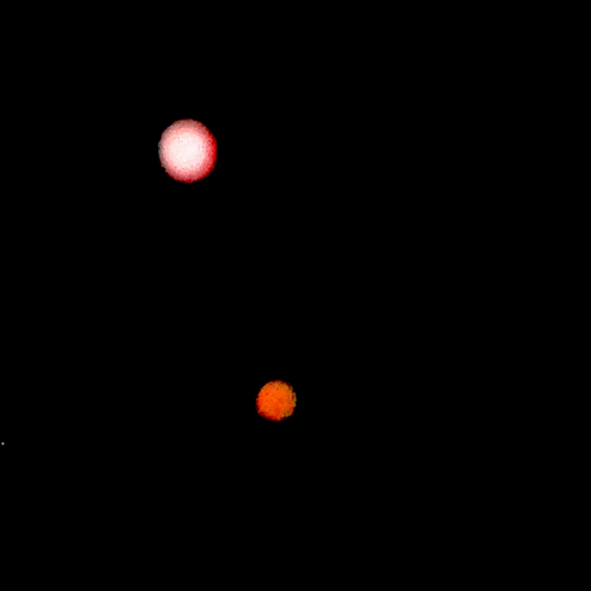
\includegraphics[height=.40\textheight]{Image.png}\\}

{The following parameters are available for formating:\\}

\begin{itemize}
\item height
\item width or length
\end{itemize}


{Note that this will not put an figure environment in \LaTeX\ 
files, so the image won't float this way. For this to
achieve to have to put \% image, \%img or \%figure before the
line.\\}

\begin{verbatim}
  %image
  Image.png
  % width = 40%
  % caption = "Moon and Mars"
\end{verbatim}


\begin{figure}[hbt]
%%
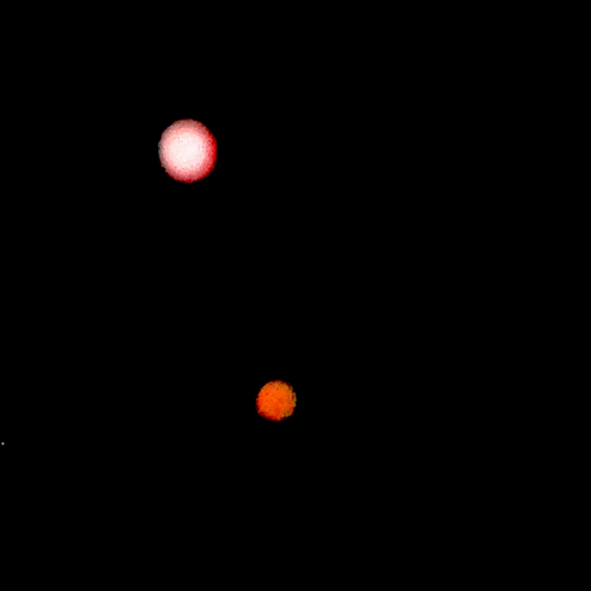
\includegraphics[width=.40\linewidth]{Image.png}
\caption{"Moon and Mars"}
\end{figure}


{This also gives you two more parameters to use:\\}

\begin{itemize}
\item name or label
\item caption
\end{itemize}


\section{Colors}

{The following colors are accepted as argument to parameters
for color or background:\\}

\colorbox{gray!75}{\parbox{\linewidth}{%%
\begin{itemize}
\item gray
\item \textcolor{green}{green}
\item \textcolor{LightYellow1}{yellow}
\item \textcolor{PaleTurquoise1}{blue}
\item \textcolor{red}{red}
\item \textcolor{white}{white}
\end{itemize}

}
}

\section{Line breaks}

{Line breaks within paragraphs are normally removed, if the
paragraph is not marked to be verbatim. To keep the line
breaks, just add \texttt{\% breaks lines} or \texttt{\% br} after the paragraph.\\}

\begin{verbatim}
       Shall I compare thee to a summer’s day?
       Thou art more lovely and more temperate:
       Rough winds do shake the darling buds of May,
       And summer’s lease hath all too short a date:
       % break lines
\end{verbatim}


{Sometime too hot the eye of heaven shines,\\
And often is his gold complexion dimmed;\\
And every fair from fair sometime declines,\\
By chance, or nature’s changing course, untrimmed:\\\\}

{\raggedleft%%
(\emph{William Shakespeare})\\}

\part{Customization}

{It is possible to customize LaFiC in various ways.\\}

\section{Templates}

{LaFiC uses templates for \LaTeX\  and HTML output. These
templates are locates in the \texttt{/templates} subdirectory of the
\texttt{/LaFiC} directory. The suffix of these files is .tmp.tex for
\LaTeX\  and .tmp.html for HTML output.\\}

{You can create your own templates an place them there. LaFiC
requires for \LaTeX\  templates at least the \texttt{graphicx} package
for images, \texttt{hyperref} for links and \texttt{xcolor} with \texttt{x11names, dvipsnames}*
and \texttt{svgnames} option for color support:\\}

\begin{verbatim}
	\usepackage{graphicx}
	\usepackage[x11names, dvipsnames*, svgnames]{xcolor}
	\usepackage[hyperindex=false, pdfpagelabels,
                    pageanchor, hyperfootnotes=false, bookmarksopen,
	    	    pdfpagemode=UseOutlines]{hyperref}
\end{verbatim}


{The templates are called by putting it's name without suffix
in the very first line of a document with a leading \% char:\\}

\begin{verbatim}
       % template
\end{verbatim}


{It is also possible to create a template for a specific
document. Such templates must be placed in the same
directory as the document and have the same basename:\\}

\begin{verbatim}
	$ ls -1
  	.
  	..
  	Beispiel.LaFiC
  	Beispiel.tmp.tex
  	Beispiel.tmp.html
\end{verbatim}


{The templates must contain placeholders for metadata like
title and author and for the content of the document.\\}

{For \LaTeX\  that would be \%TITLE\% and \%TEXT\%:\\}

\begin{verbatim}
	\documentclass{article}
	 …
	%TITLE%
	\begin{document}
	%TEXT%
	\end{document}
\end{verbatim}


{For Html it's <!-- TITLE~--> and <!-- TEXT~-->:\\}

{In Html-Vorlagen heißen die Platzhalter <!-- TITLE~--> und
<!-- TEXT~-->:\\}

\begin{verbatim}
	<html>
       	<head>
		<!-- TITLE -->
       	</head>
       	<body>
		<!-- TEXT -->
       	</body>
	</html>
\end{verbatim}


\section{Advanced: Custom keywords}

{By creating custom \LaTeX\  environment and macros as well as
the corresponding css classes, you can use your own
keywords.\\}

{Look in the \texttt{/examples} subdirectory for inspiration.\\}

\section{Stylesheets}

{In the \texttt{/styles} subdirectory there is a \texttt{standard.css} file,
which contains the CSS stylesheet used by the standard HTML
templates for LaFiC. You can place your own stylesheets here
to refer to them from custom templates. For now you have to
manually copy or link the \texttt{/styles} directory to your working directory.\\}

\section{\texttt{LaFiC.config.pl}}

{In this file in the LaFiC directory you set some
preferences. At the moment this are just two:\\}

\begin{itemize}
\item \texttt{lang} where you have the option to set another \texttt{lang}uage
then English as your preferred \texttt{lang}uage. At the moment the
only option here is \texttt{de\_DE} for German, as this is my first
\texttt{lang}uage.
\item \texttt{author} is for now the only way to specify the
\texttt{author}'s name for your LaFiC documents. I hope to provide an
in-document option soon.
\end{itemize}


{The content of this document is actually a perl construct an
must be written in the form:\\}

\begin{verbatim}
     	key => "value",
\end{verbatim}


{Please observe the comma at the end of each line.\\}

\end{document}

%%% Local Variables:
%%% mode: latex
%%% TeX-master: t
%%% End:
